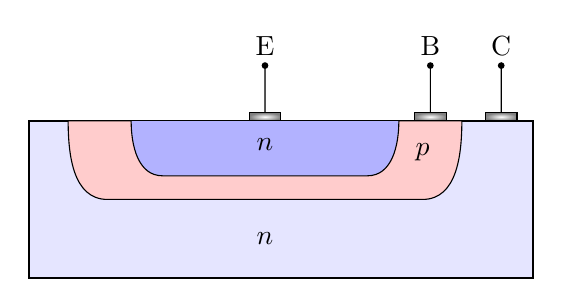
\begin{tikzpicture}
  \draw[fill] (2.1,1) -- ++(0,0.7) circle (1pt) node[above]{B};
  \draw[fill] (0,1) -- ++(0,0.7) circle (1pt) node[above]{E};
  \draw[fill] (3,1) -- ++(0,0.7) circle (1pt) node[above]{C};
  \shadedraw[color=black,fill=gray,inner color=white,outer color=gray] (1.9,1) rectangle (2.3,1.1);
  \shadedraw[color=black,fill=gray,inner color=white,outer color=gray] (-.2,1) rectangle (.2,1.1);
  \shadedraw[color=black,fill=gray,inner color=white,outer color=gray] (2.8,1) rectangle (3.2,1.1);
  \draw[fill=blue!10,thick] (-3,-1) rectangle (3.4,1);
  \draw[fill=blue!30] (-2,0.2) rectangle (2,1);
  \draw[fill=red!20] (-2.5,1) to[out=270,in=180]
    (-2,0) -- (2,0) to[out=0,in=270]
    (2.5,1) -- (1.7,1) to[out=270,in=0]
    (1.3,0.3) -- (-1.3,0.3) to[out=180,in=270] 
    (-1.7,1) -- cycle;
  \node at (0,-.5) {\(n\)};
  \node at (0,.7) {\(n\)};
  \node at (2,.6) {\(p\)};
\end{tikzpicture}
